\section{Opis technologii zastosowanych w~pracy}

% język, framework i środowisko testowe

\subsection{Ruby oraz Ruby~on~Rails} \label{technologie.baza}

\subsubsection{Ruby 1.9.3} \label{technologie.ruby}

Ruby (z.~ang.~ruby -- rubin) -- interpretowany, w~pełni obiektowy i~dynamicznie typowany język programowania stworzony w~1995 roku przez Yukihiro Matsumoto (pseudonim Matz). Wersja 1.9.2 cechuje się szybszym interpreterem, mniejszą konsumpcją zasobów oraz drobnymi poprawkami w~standardowych bibliotekach języka.

\subsubsection{Ruby~on~Rails 3.1.0} \label{technologie.ror}

Ruby~on~Rails\footnote{\url{http://rubyonrails.pl/}} (często nazywany RoR lub po~prostu Rails) to~framework open source służący do~szybkiego tworzenia aplikacji webowych stworzony głównie przez duńskiego programistę Davida Heinemeiera Hanssona w~ramach pracy nad oprogramowaniem Basecamp\footnote{Patrz: \url{http://basecamphq.com/}}. Rails to~w~pełni wyposażone środowisko do~tworzenia aplikacji internetowych opartych o~bazy danych zgodnie ze~wzorcem MVC (Model-View-Controller). Ruby~on~Rails daje programiście środowisko w~pełni oparte o~język programowania Ruby -- od~Ajax'a dostępnego w~widokach (View), do~zapytania i~odpowiedzi w~kontrolerach i~logice biznesowej modeli.


Tuż po~pojawieniu się Ruby~on~Rails na~forum publicznym okrzyknięto go~sensacyjnym. Tim O'Reilly, Założyciel O'Reilly Media mówił\footnote{Źródło: \url{http://www.rubyonrails.pl/cytaty}} ,,Ruby on Rails jest przełomem w~dziedzinie programowania aplikacji internetowych. Potężne aplikacje, których tworzenie do~tej pory zabierało tygodnie czy miesiące, są~teraz tworzone dosłownie w~kilka dni.''


Niestety -- w~ciągu ostatnich trzech lat spadło zainteresowanie technologią Ruby~on~Rails (patrz wykres \ref{fig.wykres.googleresearch}). Programiści coraz rzadziej sięgają po~ten produkt wybierając nowsze rozwiązania takie jak Django\footnote{Patrz: \url{http://www.djangoproject.com/}} napisane w~języku Python\footnote{Patrz: \url{www.python.org}}. Nadzieją na~poprawienie tej sytuacji jest nowo wydana -- trzecia wersja frameworku Ruby~on~Rails oraz~ciągły rozwój dodatków -- wtyczek \texttt{gem}. Dlatego też chcę przybliżyć tę~technologię i~zachęcić do~jej używania.

\begin{figure}[!t]
\centering
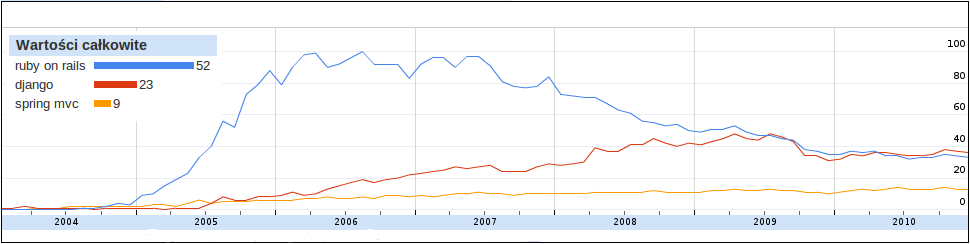
\includegraphics[width=\textwidth]{obrazki/googleresearch.png}
\caption{Statystyka wyszukiwarki Google na~temat znanych aplikacji szkieletowych (źródło: \url{http://www.google.com/insights/search/\#cat=5\&q=Ruby\%20on\%20Rails\%2CDjango\%2CSpring\%20MVC\&cmpt=q}).}
\label{fig.wykres.googleresearch}
\end{figure}

Liczby na~wykresie \ref{fig.wykres.googleresearch} wskazują, ile wyszukiwań przeprowadzono na~podstawie określonego hasła w~porównaniu do~łącznej liczby wyszukiwań przeprowadzonych w~Google w~tym czasie. Wartości te~nie odzwierciedlają bezwzględnej liczby wyszukiwań, ponieważ dane są~znormalizowane i~przedstawione na~skali od~0 do~100. Każdy punkt na~wykresie jest dzielony przez wartość najwyższego punktu. Jeśli ilość danych jest za~mała, podawana jest wartość 0. Liczby wyświetlane nad wykresem obok wyszukiwanych haseł stanowią podsumowania lub wartości łączne\footnote{Źródło: \url{http://www.google.com/support/insights//bin/answer.py?hl=pl\&answer=87285}}.

\subsubsection{RSpec + Cucumber}

RSpec\footnote{\url{http://rspec.info/}} to~narzędzie do~testownia oprogramowania pod względem testów jednostkowych oraz~behawioralnych przydatne w~realizowaniu projektów Test Driven Developement oraz~Behavior Driven Developement. Narzędzie Cucumber\footnote{\url{http://cukes.info/}} pozwala na~testowanie oprogramowania na podstawie tzw. scenariuszy -- dokumentów napisanych w języku naturalnym opisujących krok po~kroku funkcjonalności projektu.

% gemy, rozszerzenia, pluginy, dodatki, etc.

\subsection{Gemy i pluginy} \label{technologie.gemy}

\begin{enumerate}
  \item \texttt{haml}\footnote{\url{http://haml-lang.com/}} + \texttt{sass}\footnote{\url{http://sass-lang.com/}} -- plugin obsługujący język znaczników HAML używany do~prostego i~przejrzystego opisywania dokumentów XHTML oraz~CSS.
  \item \texttt{device}\footnote{\url{https://github.com/plataformatec/devise}} -- system obsługi autentyfikacji użytkowników (rejestracja, sesje, zarządzanie hasłami itp.).
  \item \texttt{thinking-sphinx}\footnote{\url{http://freelancing-god.github.com/ts/en/}} -- potężny silnik wyszukiwania i~dopasywania danych do podanych wzorców w~relacyjnych bazach danych.
  \item \texttt{will\_paginate}\footnote{\url{https://github.com/mislav/will\_paginate/wiki}} -- plugin obsługujący paginację stron.
  \item \texttt{tiny\_mce}\footnote{\url{http://tinymce.moxiecode.com/}} -- plugin pozwalający na~użycie wewnętrznego edytora HTML.
  \item \texttt{sqlite3}\footnote{\url{http://www.sqlite.org/}} -- adapter bazy danych Sqlite w~wersji trzeciej.
\end{enumerate}

% technologie webowe

\subsection{Technologie W3 i poboczne} \label{technologie.web}

\begin{enumerate}
  \item \texttt{XHTML5}\cite{html5doc} (z~ang.~HyperText Markup Language version 5 -- język znaczników hipertekstu w~wersji piątej). XHTML5 jest językiem określającym strukturę stron internetowych. Składniowo bazuje on~na~języku XML (jest podzbiorem języka XML). Wersja piąta zapewnia kompatybilność wsteczną względem poprzednich wersji, a~przy tym precyzuje niejasności wersji 4 powodujące nieoczekiwane zachowanie w~niektorych przeglądarkach.
  \item \texttt{CSS3}\cite{css3doc} (z~ang.~Cascade Style Sheet version 3 -- kaskadowy arkusz styli w~wersji trzeciej). CSS3 jest językiem określającym wygląd elementów języka XML jaki wyświetlany jest w~przeglądarce. Wersja 3 zapewnia kilka dodatkowych opcji, jak np. grid layouts (szablony pozycjonowane na bazie siatki)\footnote{\url{http://www.w3.org/TR/css3-grid/}}, shadows and rounded borders (cienie obiektów, zaokrąglenia obramowania)\footnote{\url{http://www.w3.org/TR/css3-background/}}, itp.
  \item \texttt{JavaScript} -- jest małym, lekkim, zorientowanym obiektowo wieloplatformowym językiem skryptowym. JavaScript, mimo że nie jest użyteczny jako samodzielny język, został stworzony z myślą o łatwym zagnieżdżaniu w innych produktach i aplikacjach, jak na przykład przeglądarki internetowe. JavaScript może zostać powiązany z wewnętrzną strukturą danego środowiska dając programiście swobodną kontrolę nad jego elementami.

  \item \texttt{AJAX} (z~ang. Asynchronous JavaScript and XML, asynchroniczny JavaScript i~XML) -- technologia tworzenia aplikacji internetowych, w~której interakcja użytkownika z~serwerem odbywa się bez przeładowywania całego dokumentu, w~sposób asynchroniczny. Ma~to~umożliwiać bardziej dynamiczną interakcję z~użytkownikiem niż w~tradycyjnym modelu, w~którym każde żądanie nowych danych wiąże się z~przesłaniem całej strony HTML.

  \item \texttt{jQuery}\footnote{\url{http://docs.jquery.com/Main\_Page}} (z.~ang. query -- zapytanie) -- lekka biblioteka programistyczna dla języka JavaScript, ułatwiająca korzystanie z~JavaScript (w~tym manipulację drzewem DOM). Kosztem niewielkiego spadku wydajności w~stosunku do~profesjonalnie napisanego kodu w~niewspomaganym JavaScripcie pozwala osiągnąć interesujące efekty animacji, dodać dynamiczne zmiany strony, wykonać zapytania AJAX. Większość pluginów i~skryptów opartych o~jQuery działa na~stronach nie wymagając zmian w~kodzie HTML (np.~zamienia klasyczne galerie złożone z~miniatur linkujących do~obrazków w~dynamiczną galerię). Wszystkie efekty osiągnięte z~pomocą jQuery można osiągnąć również bez jej użycia. Jednak kod okazuje się nieporównywalnie dłuższy i~bardziej skomplikowany.
\end{enumerate}
